Calcular la masa que posee una rueda cuya velocidad tiene una magnitud de 19 m/s y su energía cinética es de 1000 J.

\begin{minipage}{0.65\textwidth}
    \begin{solutionbox}{8cm}
        \begin{multicols}{2}
            Datos:

            Ec = 1000 J

            v = 19 m/s

            m = ?

            La energía cinética es:
            \[E_c=\frac{1}{2}mv^2\]

            Despejando a "m"

            \[m=\dfrac{2E_c}{v^2}\]

            \vspace{2cm}

            Sustituyendo nuestros datos en la fórmula:

            \[
                \begin{array}{rl}
                    m & =\dfrac{2E_c}{v^2}                                              \\[1em]
                      & =\dfrac{2(1000J)}{(19 \text{ m/s})^2}                           \\[1em]
                      & =\dfrac{2000 \text{ kg m$^2$/s$^2$}}{(361 \text{ m$^2$/s$^2$})} \\[1em]
                      & =5.54 \text{ kg}
                \end{array}
            \]






        \end{multicols}
        \begin{center} Obtenemos que la masa es de 5.54 kg.\end{center}
    \end{solutionbox}
\end{minipage}\hfill
\begin{minipage}{0.3\textwidth}
    \begin{figure}[H]
        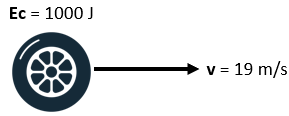
\includegraphics[width=\linewidth]{../images/energia_cinetica_problema_3.png}
    \end{figure}
\end{minipage}